\scanpage{115}
\mspage{2}

We introduce vertices
\[
(6)\qquad R_r^{i,j}\qquad r\in\mathcal{R},\quad (i,j)\in\operatorname{Rep}\{0,1,\infty\}\quad\text{i.e. }i,j\in\{0,1,\infty\},\ i\ne j
\]
as indi\uline{cated, satisfying} only the relations
\[
(7)\qquad
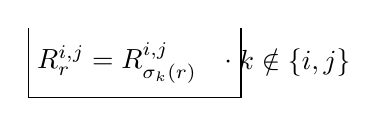
\begin{tikzpicture}[baseline=(relation.base)]
  \node[inner xsep=3pt,inner ysep=5pt] (relation)
    {$R_r^{i,j}=R_{\sigma_k(r)}^{i,j}\quad\cdot$};
  \draw[line width=.45pt] (relation.north west) -- (relation.south west)
    -- (relation.south east) -- (relation.north east);
  \node[anchor=west,inner sep=0pt,xshift=-1pt] at (relation.east)
    {$k\notin\{i,j\}$};
\end{tikzpicture}
\]
We say that $R_r^{ij}$ is ``close'' to the
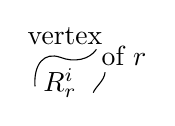
\begin{tikzpicture}[baseline=(baseR.base)]
  \node[anchor=base west,inner sep=0pt] (baseR) at (0,0) {$R_r^i$};
  \node[anchor=base west,inner sep=0pt] at (-.20,.59) {\inserted{vertex}};
  \node[anchor=base west,inner sep=0pt] at (.74,.33) {\inserted{of $r$}};
  \draw[line width=.4pt] (-.10,.06) .. controls (-.12,.35) and (.02,.50) .. (.22,.43)
    .. controls (.40,.36) and (.59,.40) .. (.68,.53);
  \draw[line width=.4pt] (.79,.24) .. controls (.78,.13) and (.67,.06) .. (.64,-.02);
\end{tikzpicture}
($=R_s,R_o,R_f$ according as $i=0,1,\infty$), it lies on the side
\deleted{\unsure{of the nearest}} \inserted{which joins this one}
\deleted{\illegible{1} \unsure{reference} opposite} to the vertex of type $j$.

We introduce arcs
\[
(8)\qquad \lambda_r^i:R_r^{i,i+1,}\longrightarrow R_r^{i,i+2}\qquad r\in\mathcal{R},\ i\in\{0,1,\infty\}
\]
\[
(9)\qquad a_r^i:R_r^{i\deleted{\unsure{+2|i+2}},i+1}\longrightarrow R_r^{i+1,i+2}\qquad r\in\mathcal{R},\ i\in\{0,1,\infty\}
\]
\margin{\uline{NB} We write for simplicity $i+1$ instead of the result of the cyclic permutation $(0,1,\infty)\longmapsto(1,\infty,0)$, i.e. we identify $\{0,1,\infty\}$ with $\mathbb{Z}/3\mathbb{Z}\ldots$}

\deleted{which}
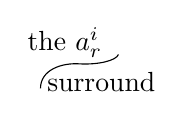
\begin{tikzpicture}[baseline=(entourent.base)]
  \node[anchor=base west,inner sep=0pt] (entourent) at (0,0) {surround};
  \node[anchor=base west,inner sep=0pt] at (-.25,.52) {\inserted{the $a_r^i$}};
  \draw[line width=.4pt] (-.08,.04) .. controls (-.08,.27) and (.18,.37) .. (.43,.35)
    .. controls (.65,.34) and (.88,.39) .. (.91,.47);
\end{tikzpicture}
the reference flag $r$ forming a closed contour in the direction
\deleted{\uline{opposite}} \inserted{of} the orientation of $r$ ---
\deleted{on the other hand} \inserted{\unsure{of = denote}} the $\lambda_r^i$
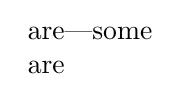
\begin{tikzpicture}[baseline=(oldverb.base)]
  \node[anchor=base west,inner sep=0pt] (oldverb) at (0,0) {\deleted{are}};
  \node[anchor=base west,inner sep=0pt] at (0,.43) {\inserted{\unsure{are|some}}};
\end{tikzpicture}
\deleted{\unsure{a}} portions of arc turning around the vertices of $r$ of type $i$
in the direction corresponding to the orientation of $r$.
(This \deleted{\unsure{to us}} seems preferable to the reverse notational convention).
We have only the \deleted{identities} redundancies
\[
(10)\qquad \boxed{a_r^i=a_{\tau_i(r)}^i}
\]
\margin{\begin{tabular}{@{}l@{}}
\uline{NB} We denote\\
by the \deleted{\unsure{these}} letters\\
the arrows obtained\\
after filling in\\
certain holes\\
if we fill in\\
$R_r^i$,
\end{tabular}}
\margin{\begin{tabular}{@{}l@{}}
(\uline{NB} if\\
the disks where\\
$\lambda_r^i$ becomes $=1$)
\end{tabular}}

\deleted{We denote}

\uline{NB} We shall suppose that the combinatorial map is realized by its canonical conformal realization, which is a real analytic surface $\unsure{\mathbb{C}|\mathcal{C}}$ hence $C^\infty$, of which we can consider its blow-up at the $R_\varphi$ $(\varphi\in S)$ and the cutting of the blow-up, which is a real analytic surface with boundary (but not conformal) whose interior coincides with $X\setminus S$, we denote it

\mspage{114}
